\documentclass{llncs}
\bibliographystyle{plain}
\newcommand{\tab}{\hspace*{2em}}
\usepackage[english]{babel}
\usepackage{amssymb,amsmath,graphicx,mdwlist,paralist,multirow,array,color}
\usepackage[noend]{algpseudocode}
\usepackage{chngpage,url,algorithm,algorithmicx}

\renewcommand{\algorithmicforall}{\textbf{for each}}
%\algrenewcommand{\algorithmiccomment}[1]{\hfill$\blacktriangleright$ #1}

\begin{document}

\title{Time Division Multiplexing of Network Access by Security Groups in High Performance Computing Environments}
\author{Joshua Ferguson}
\date{\today}
\maketitle
\begin{abstract}
As the scale of data used in computation increases the utility of High Performance Computing as a Service increases in tandem. Security concerns in such a domain are still being solved using traditional Operating System mechanisms of memory protection and file access privileges ~\cite{buyya1999high}. However there exist scenarios where customers demand more intuitive and rigorously verifiable security solutions. This paper presents a robust and application transparent network security solution that is both intuitive and easily verifiable. This paper's main contribution is a mechanism designed to enforce high level time division multiplexing of network access according to security groups. By dividing network access into time windows, interactions between applications over the network can be prevented in an easily verifiable way. 
\end{abstract}
\section{Introduction}
High Performance Computing (HPC) systems are comprised of numerous individual computing systems networked and administrated together such that they can be used as a single system. Popular examples of these systems include some custom made such as the Cray I and the modern IBM Sequoia~\cite{leavitt2012big}, though more common are simple Computer Clusters in which Commercial Off The Shelf (COTS) equipment is utilized~\cite{buyya1999high}. Security within these systems is often enforced through traditional Operating System (OS) mechanisms of memory protection and file access privileges~\cite{buyya1999high}. 

\textcolor{red}{-*-*-*-*-*-BEGIN new paragraph-*-*-*-*-*-}


Application developers for this domain of systems spans a broad spectrum, ranging from undergraduate students learning concurrent programming to defence contractors executing classified simulations. Moving towards the most demanding end of the spectrum, security concerns among application-side stakeholders increase and additional methods are employed to enforce information security. At some point along this spectrum stakeholders decide physical separation to satisfy security concerns. The reasons behind this can be numerous, but likely stem from two major goals: simplicity of implementation and verification; and risk aversion/management. It is undeniable that physical separation provides a level of information security that is hard to replicate through the use of software, however the financial costs are significant - devoting entire HPC systems to running jobs sequentially. 

\textcolor{red}{-*-*-*-*-*-END new paragraph-*-*-*-*-*-}

This paper presents Time Division Multiplexing (TDM) of network access as a viable alternative to physical separation. By modulating network access between application security groups we can provide an intuitive security mechanism capable of being verified in real-time. Furthermore by implementing this mechanism at the operating system level it becomes transparent to user applications, meaning no modification to existing application code is necessary. [Mention we have built a prototype, and mention formal proof.]
\section{Related Work}
\section{Problem Definition}

We begin by defining an abstract HPC environment through which the general case of our security challenge is shown.
\subsection{An Abstract HPC Environment}
\begin{figure}
\centering
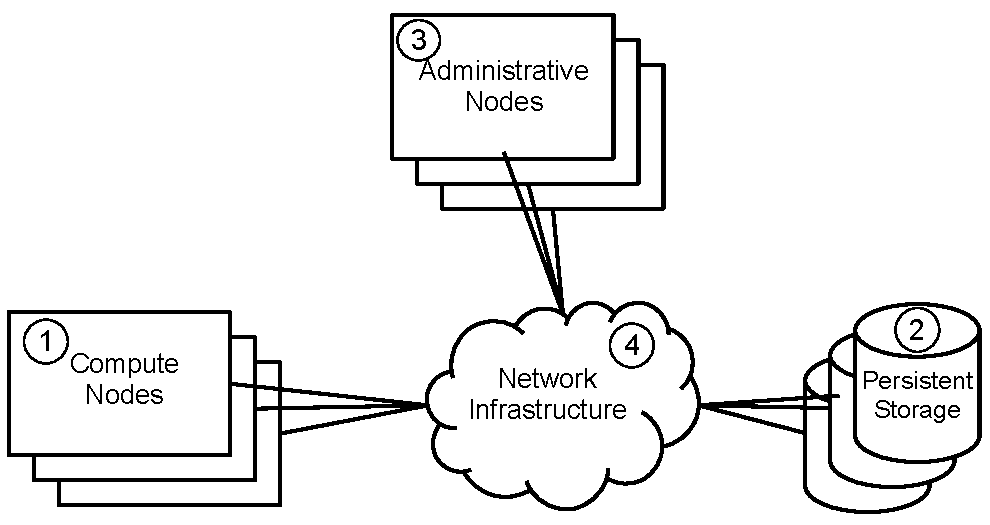
\includegraphics[scale=0.5]{abstract_hpc_environment.pdf}
\caption{An abstract HPC environment.}
\label{fig:abstract_hpc_environment}
\end{figure}
There are four basic resources in most HPC systems represented in Figure~\ref{fig:abstract_hpc_environment} as: 
\begin{enumerate} \itemsep1pt \parskip0pt \parsep0pt
\item \textbf{compute nodes} - independent computing devices designated to run user submitted applications. These devices are capable of storing temporary data locally. They send and receive data across network infrastructure for three main purposes:\begin{inparaenum}[\itshape a\upshape)]
\item storing or accessing data on the persistent storage devices;
\item relaying data between other compute nodes working in tandem on the same user application;
\item and sending or receiving commands (or reports, as the case may be) from the administrative nodes, through which users interact.
\end{inparaenum}
\item \textbf{persistent storage} - storage devices (usually of much higher capacity than the compute nodes) capable of storing large quantities of user application data. User data is commonly co-located across disks using RAID (redundant array of inexpensive disks) technology ~\cite{katz1989disk} for higher storage efficiency and redundancy. 
\item \textbf{administrative nodes} - computing devices where \begin{inparaenum}[\itshape a\upshape)]
\item both administrators and users interact with the system, common tasks of which include issuing job or system commands, accessing reports and results, and performing maintenance;
\item resource management software is centrally located and executed ~\cite{keller2001anatomy}, common examples include IBM's Tivoli Workload Scheduler and the MOAB Cluster Suite by Adaptive Computing \cite{arackal2009access}\cite{jackson2006demand}.
\end{inparaenum}
\item \textbf{network infrastructure} - devices facilitating the transmission of data between nodes within the HPC system. Mediums vary widely and include copper, optical, and wireless. The most common technologies used in HPC environments are Ethernet and InfiniBand \cite{bozzo2006design}\cite{madai2010performance}. 
\end{enumerate}
\subsection{System Assumptions}
\subsection{Security Challenge}

\begin{table}
\begin{adjustwidth}{-4em}{-4em}
\centering
\begin{tabular}{ccc|c|c|}
& & \multicolumn{3}{ c }{\textbf{Solutions}} \\ \cline{3-5}
\centering\arraybackslash \textbf{Hardware Location} &  \multicolumn{1}{ c| }{\centering\arraybackslash \textbf{Security Challenge}} & \multicolumn{1}{ b{1.65cm}| }{\centering\arraybackslash Board Separation} & \multicolumn{1}{ b{.6cm}| }{\centering\arraybackslash IME} & \multicolumn{1}{ b{1.97cm}| }{\centering\arraybackslash Posix \hspace{2em}Permissions}   \\ \cline{1-5}
\multicolumn{1}{ |c| }{\multirow{2}{*}{Compute Nodes} } &
\multicolumn{1}{ |p{5cm}| }{\centering\arraybackslash Local Data Storage} & \checkmark &   & \checkmark         \\ \cline{2-5}
\multicolumn{1}{ |c  }{}                        &
\multicolumn{1}{ |p{5cm}| }{\centering\arraybackslash Local Data Processing} & \checkmark &   &  \checkmark        \\ \cline{1-5}
\multicolumn{1}{ |c|  }{Persistent Storage}  &
\multicolumn{1}{ |p{5cm}| }{\centering\arraybackslash Co-location of user data} &  &  \checkmark & \checkmark   \\ \cline{1-5}
\multicolumn{1}{ |c|  }{Administrative Node}  &
\multicolumn{1}{ |p{5cm}| }{\centering\arraybackslash Accept and Schedule User Jobs} &   &   & \checkmark   \\ \cline{1-5}
\multicolumn{1}{ |c|  }{\multirow{6}{*}{Network Infrastructure}} &
\multicolumn{1}{ |p{5cm}| }{\centering\arraybackslash Transmit intra-application data between compute nodes} &   &   &       \\ \cline{2-5}
\multicolumn{1}{ |c  }{}                        &
\multicolumn{1}{ |p{5cm}| }{\centering\arraybackslash Transmit data to/from compute nodes and persistent storage} &   &   &       \\ \cline{2-5}
\multicolumn{1}{ |c  }{}                        &
\multicolumn{1}{ |p{5cm}| }{\centering\arraybackslash Transmit commands from scheduler to compute nodes} &   &   &       \\ \cline{1-5}
\end{tabular}
\caption{Security challenges and technology used to solve them}
\label{tab:security_challenges}
\end{adjustwidth}
\end{table}

The security fear of customers with sensitive data is that a different customer could, through chance or intention, acquire or manipulate their data. There exist three main mediums across which data may be exposed. 
\section{Design Goals}
Here we describe the major goals in the design and implementation of the TDM security mechanism.
\subsection{Mechanism and Policy Separation}
Envisioning the tool as enabling a more secure form of HPCaaS, the type, number, and scale of jobs assigned to any of the systems can be widely varied. To handle this, at the least, the tool must be capable of receiving and modifying policy at the start of each new job. Furthermore, to provide more fine-grained control an online policy modification scheme is desirable for managing performance tradeoffs between security groups. We define the mechanism and policy split of our tool to be an ability to receive and actuate policy changes at the finest granularity in which the tool operates. [Mechanism Policy split is really along the difference between the formal notion that nodes must be transparently separated from the medium and how it is accomplished (with a queue, at the TCP layer, on ethernet, etc.)]
\subsection{Network Fabric Agnostic}
Two major technologies are used to network HPC systems: Ethernet and InfiniBand. Any tool for improving security across the broad spectrum of HPC systems must be capable of operating in each. Further, numerous network topologies exist within these technologies; switched fabric and tree structures are the most common for InfiniBand and Ethernet, respectively. For our purposes we define this tool to be network fabric agnostic if the tool is conceptually capable of being implemented in either Ethernet or InfiniBand networks. 
\subsection{User Application Transparent}
A fundamental requirement of the tool is that it be transparent to user applications. Applications written for HPC environments are often quite complex and it is likely that customers would be reluctant to make even minor modifications, especially to programs written in the past that are under re-use. For our purposes we define user application transparency as the ability to run an application without modification to successful end on an HPC system using our tool, given that it can also do so on a system not using our tool. 
\subsection{Provably Secure}
The final and most important requirement of this tool is that it provably perform its task. 
\section{Implementation}
As a proof of concept we have implemented a version of the tool for the Linux operating system using C++11. In this section we will describe the tool's architecture, operation, and how it adheres to the design goals from the previous section.
\subsection{Overview}
\begin{algorithm}
	\caption{Window Controller opening and closing network access windows.}
	\label{alg:window_controller}
	\begin{algorithmic}[1]
	\Statex
	\Function{$Open\_Windows$}{$Scheduler$}
		\State $Scheduler.initialize();$
		\While{$End\_Command\_Not\_Received$}
			\State $Security\_Group \gets Scheduler.get\_next\_group();$
			\State $Security\_Group.state \gets \textsc{state.open};$
			\ForAll {$node \in Security\_Group$}
				\State $send(node.address,$ \par
	        \hskip\algorithmicindent\hspace{3em} $Security\_Group.crypto\_sign(\textsc{command.open}));$
        \State $node.state \gets \textsc{state.open};$
			\EndFor
			\While{$Security\_Group.state == \textsc{state.open}$}
				\State $node\_response \gets block\_on\_receive\_message();$
				\If{$node\_response.state == \textsc{state.closed}$} 
					\State $node.state \gets \textsc{state.closed};$
				\Else 
					\State $\textbf{throw}\hspace{.6em} \textsc{error.unclosed\_node};$
				\EndIf
				\State $Security\_Group.state \gets \textsc{state.closed};$
				\ForAll {$node \in Security\_Group$}
					\If{$node.state == \textsc{state.open}$}
						\State $Security\_Group.state \gets \textsc{state.open};$
					\EndIf
				\EndFor
				
			\EndWhile
		\EndWhile

	\EndFunction

	\end{algorithmic}
\end{algorithm}

\begin{algorithm}
	\caption{Node Control Mechanism opening and closing access to the network.}
	\label{alg:node_controller}
	\begin{algorithmic}[1]
		\Statex
		\Function{$Node\_Control\_Mechanism$}{}
			\State $Queue \gets initialize\_queue;$
			\While{$exit\_command\_not\_received$}
				\State $state \gets Close\_Network\_Access(Queue);$
				\While {$open\_command\_not\_received$}
					\State $message \gets block\_on\_receive\_message();$
				\EndWhile
				\State $state \gets Open\_Network\_Access(Queue);$
				\State $sleep(message.time);$
				\State $state \gets Close\_Network\_Access(Queue);$
				\State $send\_acknowledgement(state);$
			\EndWhile
		\EndFunction
		\Statex
		\Function{$Close\_Network\_Access$}{$Queue$}
			\State $state.egress \gets Network\_Egress.enqueue(Queue);$
			\State $state.ingress \gets Network\_Ingress.drop\_packets();$
			\State \Return{$state$}
		\EndFunction
		\Statex
		\Function{$Open\_Network\_Access$}{$Queue$}
			\State $state.ingress \gets Network\_Ingress.accept\_packets();$
			\State $state.egress \gets Queue.process\_packets\_to\_network();$
			\State \Return{$state$}
		\EndFunction
	\end{algorithmic}
\end{algorithm}	
		
The tool is composed of four major components:  the window scheduler, ingress controller, egress controller, and the state controller. The window scheduler can be located on any administrative node within the system, preferably co-located with the system job scheduler. The remaining controllers are located throughout the HPC environment, with a copy on each compute node that is designated to execute user applications. 

The system provides enhanced security by time dividing access to the network according to security groups. As jobs are scheduled on the system, the window scheduler must be informed of the intended location and their assigned security group. As jobs are run on compute nodes throughout the system the window scheduler communicates with the state controller on each node to designate time windows. During any individual time window only one security group has authorization to access the network. For any given time window in which a security group does not have access to the network, outgoing network packets are stored in a local queue while incoming packets are just ignored and deleted. The window scheduler is tasked with alternating time window authorization between security groups.

The following subsections describe each components operations in further detail. 
\subsection{State Controller}
The state controller has three major tasks:
\begin{enumerate} \itemsep1pt \parskip0pt \parsep0pt
\item Securely send and receive communication with the window scheduler for the system
\item Transit both the ingress and egress controllers between states of network access and denial
\item Collect and store performance data on the egress queue's memory usage
\end{enumerate}

 

\subsection{Ingress Controller}
The ingress controller is a firewall of incoming network packets and has two states:
\begin{enumerate} \itemsep1pt \parskip0pt \parsep0pt
\item Open access of network packets to applications on the node
\item Closed to network packets except for those from explicitly allowed sources (a whitelist style of firewall)
\end{enumerate}


During the open state incoming packets are processed normally. During the ingress closure, incoming packets, except those allowed by the whitelist, are dropped. The whitelist is designated to allow only necessary infrastructure communications such as Network Time Protocol (NTP), performance measurements, and especially packets from the window scheduler.
\subsection{Egress Controller}
The egress controller, similar to the ingress controller, has two major states:
\begin{enumerate} \itemsep1pt \parskip0pt \parsep0pt
\item Open flow of packets onto the network
\item Diversion of outgoing packets into a blocked queue
\end{enumerate}

\subsection{Window Scheduler}
The window scheduler has three major tasks: 

Determine system network access states for the next time window 
Validate the closure of the previous time window
Communicate the next time window states to compute nodes
To determine the network access states for the next time window the scheduler must run a scheduling algorithm on a few historical inputs. The base case scheduling algorithm is round robin (i.e., equal window size for each security group). To improve performance, a number of heuristics have been considered for the creation of a dynamic priority scheduling algorithm: the egress controller memory usage of compute nodes, number of TCP timeouts, and externally imposed priorities. 
\section{Case Study}
\begin{figure}
\centering
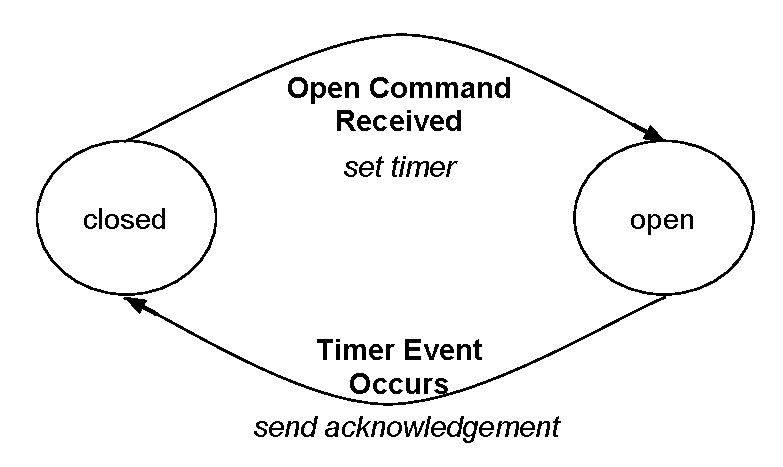
\includegraphics[scale=0.5]{node_state_diagram.pdf}
\caption{State diagram of a compute node.}
\label{fig:node_state_diagram}
\end{figure}
\begin{figure}
\centering
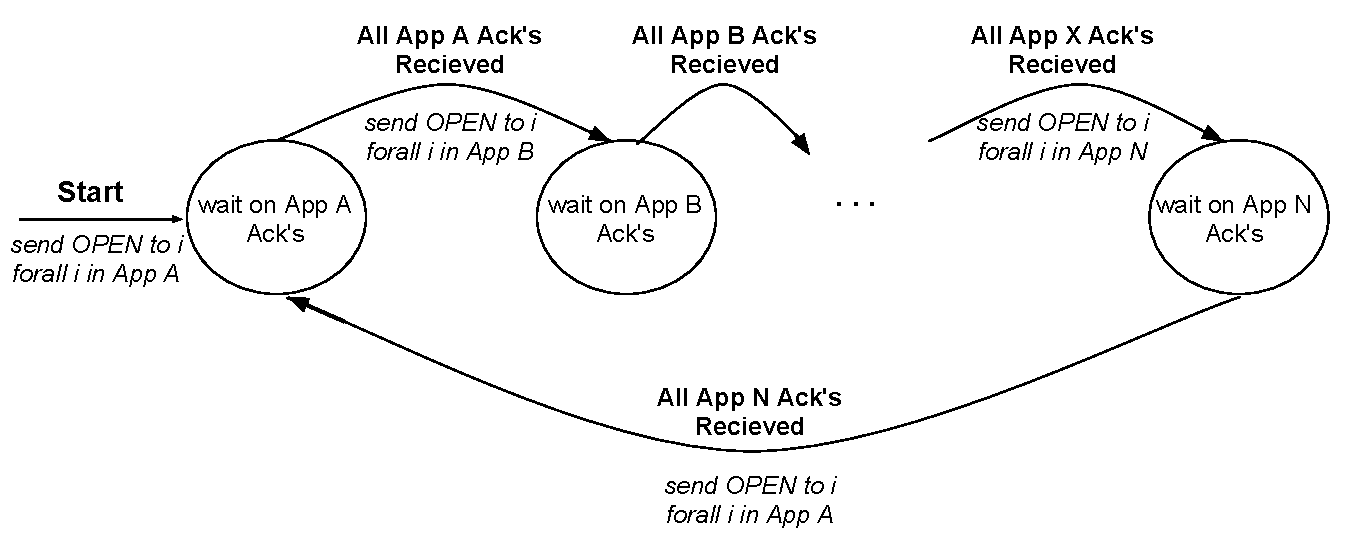
\includegraphics[scale=0.5]{control_state_diagram.pdf}
\caption{State diagram of an example window controller.}
\label{fig:control_state_diagram}
\end{figure}

\subsection{Performance}
\subsection{Security Validation}
\section{Conclusion}
\subsection{Further Work}
Implement dynamic scheduling algorithm on the window scheduler using memory usage statistics from compute nodes. 

\bibliographystyle{plain}
\bibliography{bibliography}

\end{document}
